\section{Introducción}

En la industria de la microelectrónica, los DSP están controlados por microprocesadores con firmware embebido, lo que permite al operario gestionarlos a través de estos últimos. Por esta razón, se propuso integrar el filtro transmisor del Laboratorio N°4 y el microprocesador del Laboratorio N°5 en un solo diseño. De esta forma, todo el control externo del transceptor se puede realizar a través de UART con un script de Python.

Al DSP se le debió colocar una memoria \emph{RAM} para guardar un log de la señal filtrada, como se muestra en la \autoref{fig:esq_consigna_dsp}.

\begin{figure}[H]
    \centering
    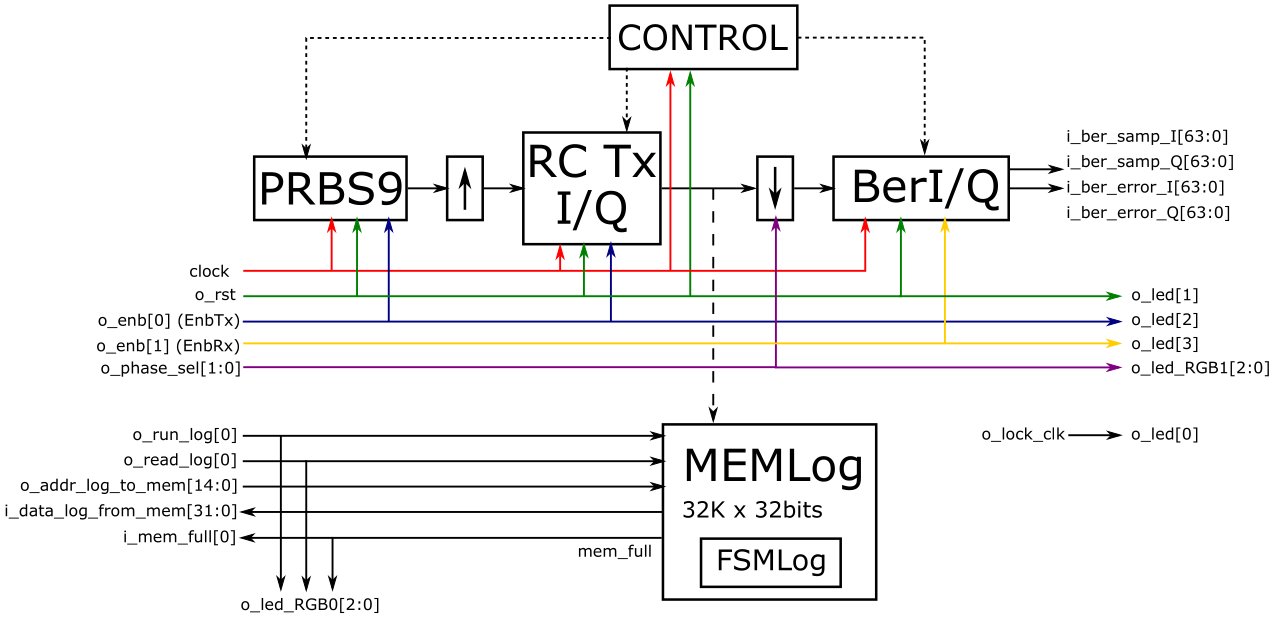
\includegraphics[width=0.9\linewidth]{img/esq_consigna_dsp.png}
    \caption{Esquema de conexión propuesto para la memoria RAM.}
    \label{fig:esq_consigna_dsp}
\end{figure}

Todas las señales de control salen de una interfaz denominada \emph{Register File} o mapa de registros, la cual es un banco de registros que almacena los comandos que provienen del microprocesador. La propuesta fue conectar este banco como se muestra en la \autoref{fig:esq_consigna_rf}. Por otro lado, los comandos que envía el microprocesador pasan por un GPIO de 32 bits, en el formato mostrado en la \autoref{fig:esq_consigna_comando}.

\begin{figure}[H]
    \centering
    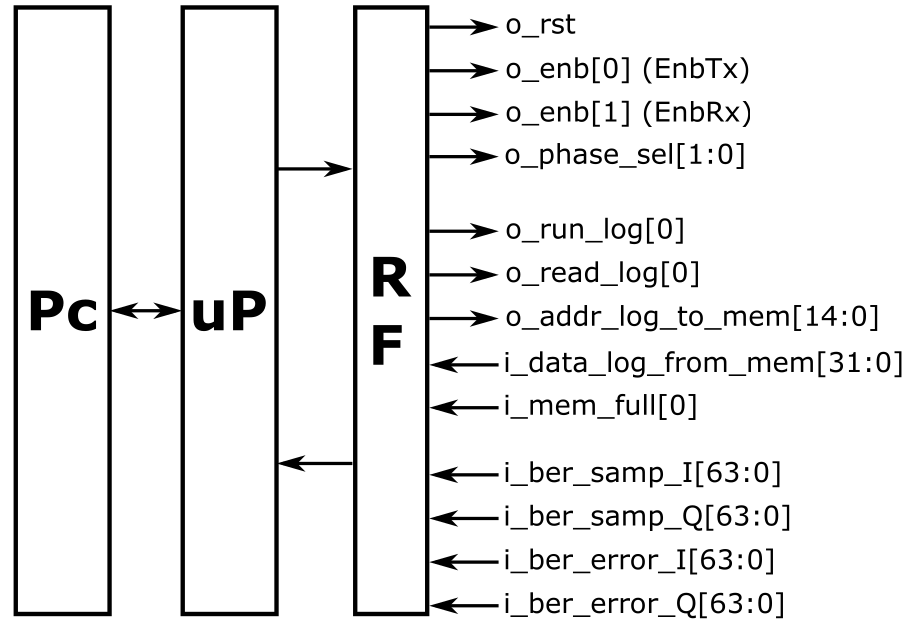
\includegraphics[width=0.4\linewidth]{img/esq_consigna_rf.png}
    \caption{Interfaz del mapa de registros.}
    \label{fig:esq_consigna_rf}
\end{figure}

\begin{figure}[H]
    \centering
    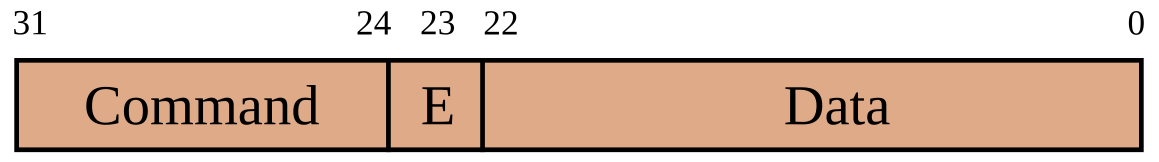
\includegraphics[width=0.5\linewidth]{img/esq_consigna_comando.png}
    \caption{Campos de la palabra a enviar por el microprocesador.}
    \label{fig:esq_consigna_comando}
\end{figure}

Con esto se espera que una PC pueda obtener un gráfico de los datos de la señal filtrada, almacenados en la memoria de logueo del DSP, además de controlar el encendido, apagado, reset, etc. del módulo.

\section{Objetivos}

Integrar el bloque de DSP y de microprocesador, ya armados anteriormente en un solo módulo, y con esto integrar además los conocimientos básicos del diseño digital.

\section{Desarrollo}

\subsection{Memoria de Logueo}

La nueva memoria que posee el transceptor se diseñó para que la herramienta Vivado infiera una Block RAM en la FPGA, para esto se escribió el RTL tomando como referencia las plantillas que posee la herramienta para sintetizar este bloque. Luego, se construyó sobre ella una máquina de estados, encargada de recibir los comandos del mapa de registros y enviar los datos correspondientes al mismo, así como se muestra en la \autoref{fig:esq_mem}. Por otro lado, el diagrama de estados se puede observar en la \autoref{fig:esq_fsm}. A pesar de que la consigna especifique una memoria de 32K, primero se intentó sintetizar el diseño con 1K y luego de terminar el diseño ir subiendo la capacidad, debido a los limitados recursos de esta FPGA.

\begin{figure}[H]
    \centering
    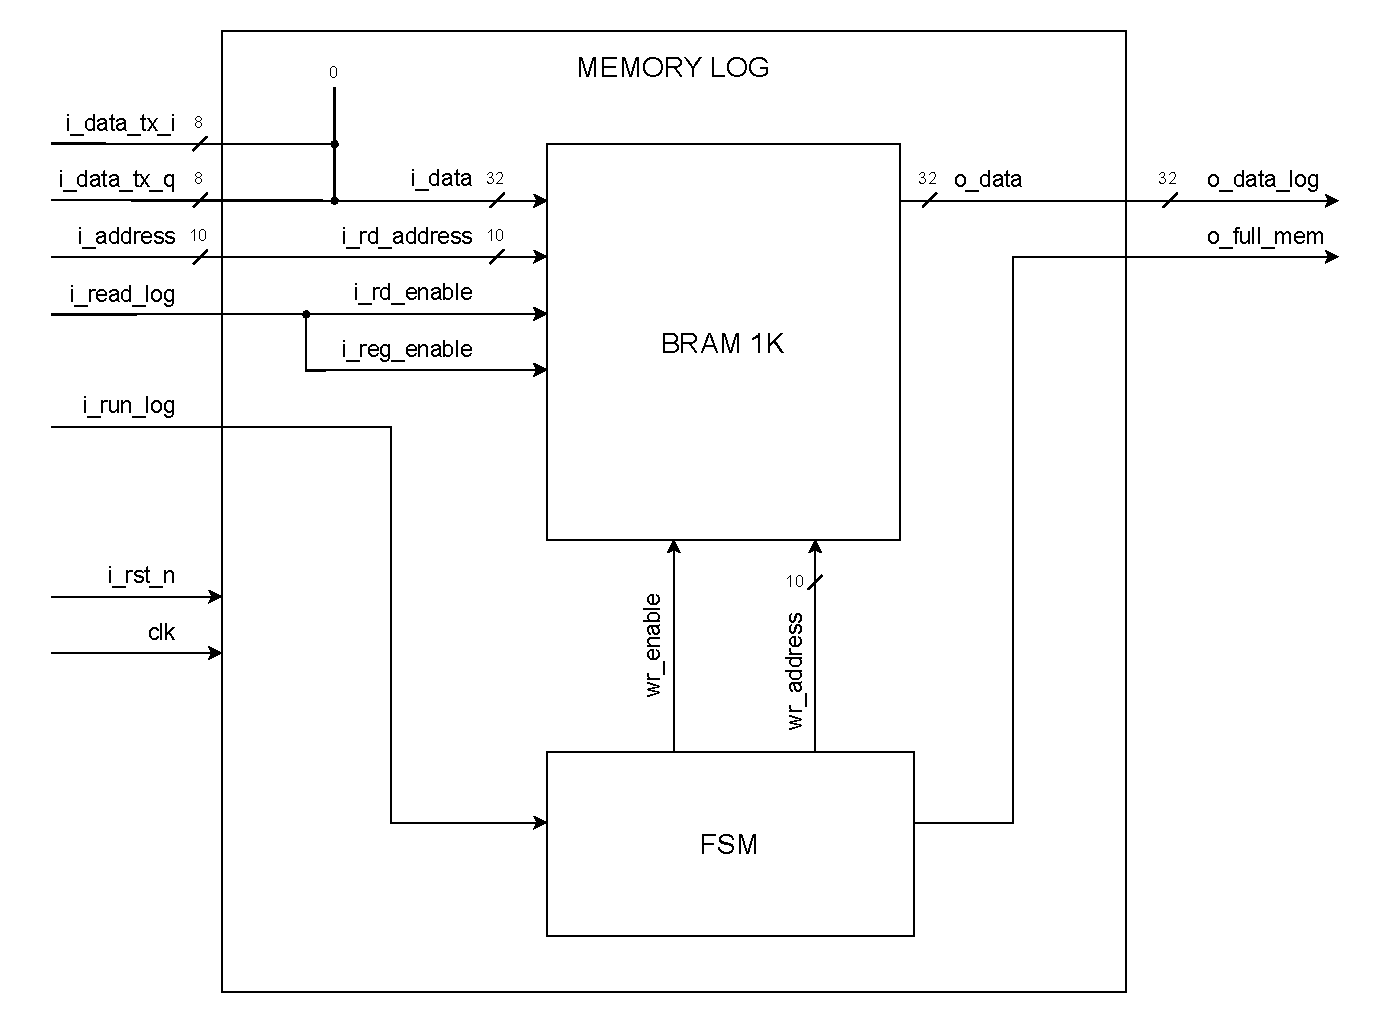
\includegraphics[width=0.8\linewidth]{img/esq_mem.pdf}
    \caption{Arquitectura de la máquina de estados con la BRAM.}
    \label{fig:esq_mem}
\end{figure}

\begin{figure}[H]
    \centering
    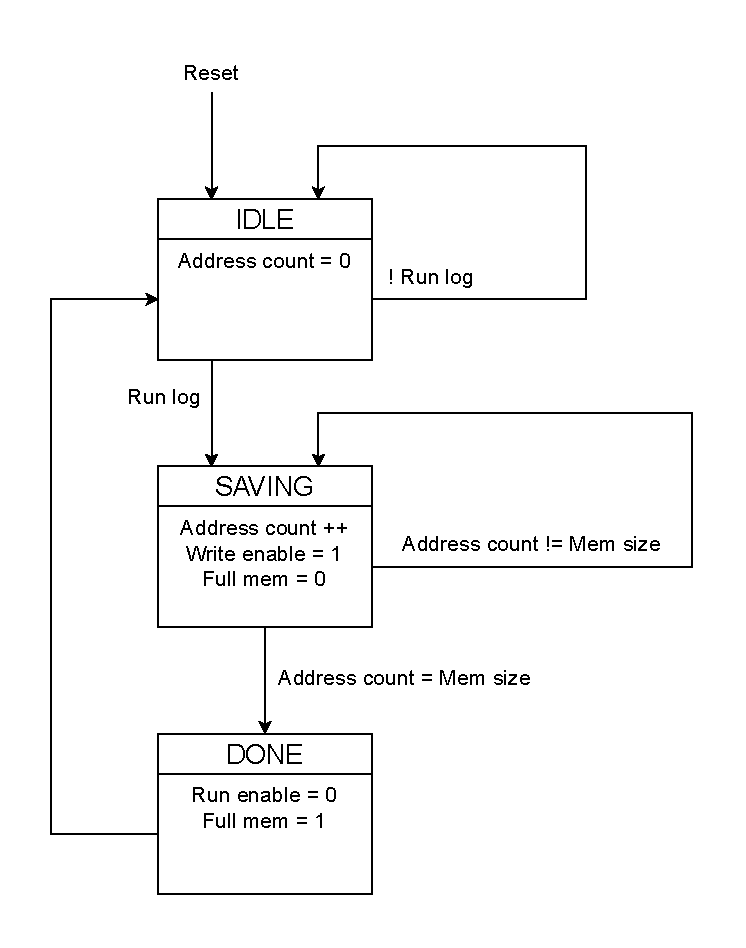
\includegraphics[width=0.5\linewidth]{img/esq_fsm.pdf}
    \caption{Diagrama de estados de la memoria.}
    \label{fig:esq_fsm}
\end{figure}

Esta nueva implementación se puso a prueba con el VIO, mostrando los resultados en la \autoref{fig:vio_mem}. Al presionar el botón \texttt{probe\_out3}, se habilitó el logueo, donde el led \texttt{probe\_in1[0]} indicó que la memoria se llenó y el led \texttt{probe\_in1[2]} se encendió y apagó para indicar que se había iniciado el proceso.

\begin{figure}[H]
    \centering

    \begin{minipage}{0.48\linewidth}
        \centering
        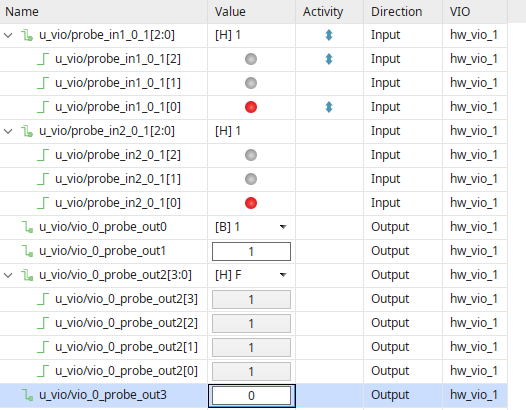
\includegraphics[width=1\linewidth]{img/vio_mem_run.png}
        \subcaption{Habilitación del logueo.}
        \label{fig:vio_mem_run}
    \end{minipage}
    \hfill
    \begin{minipage}{0.48\linewidth}
        \centering
        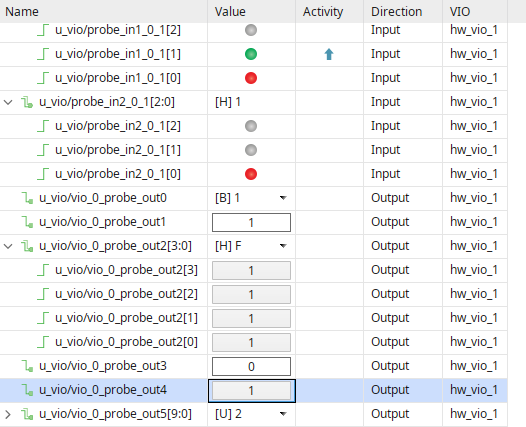
\includegraphics[width=1\linewidth]{img/vio_mem_read.png}
        \subcaption{Memoria llena.}
        \label{fig:vio_mem_read}
    \end{minipage}

    \caption{Proceso de guardado con el VIO.}
    \label{fig:vio_mem}
\end{figure}

En la \autoref{fig:ila_mem_read} se puede ver cómo la señal del canal I y Q (\texttt{probe\_1} y \texttt{probe\_2} respectivamente) cambian al usar el trigger del ILA mientras se cambia la dirección de lectura.

\begin{figure}[H]
    \centering
    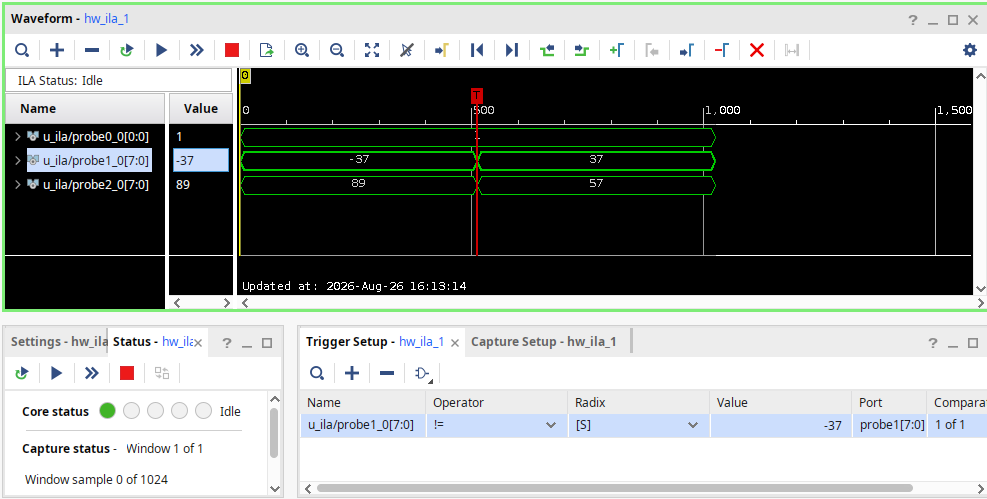
\includegraphics[width=0.8\linewidth]{img/ila_mem_read.png}
    \caption{Cambio del dato obtenido al leer otra dirección.}
    \label{fig:ila_mem_read}
\end{figure}

\subsection{Register File} \label{sec:rf}

El banco de registros se modeló según la arquitectura de la \autoref{fig:esq_rf}. En este esquema, el dato de 32 bits proveniente del GPIO es desarmado en grupos de bits para almacenarlos en registros o comandar multiplexores según corresponda. También almacena cada dato que se recibe del DSP y lo envía al GPIO dependiendo el comando que se reciba.

\begin{figure}[H]
    \centering
    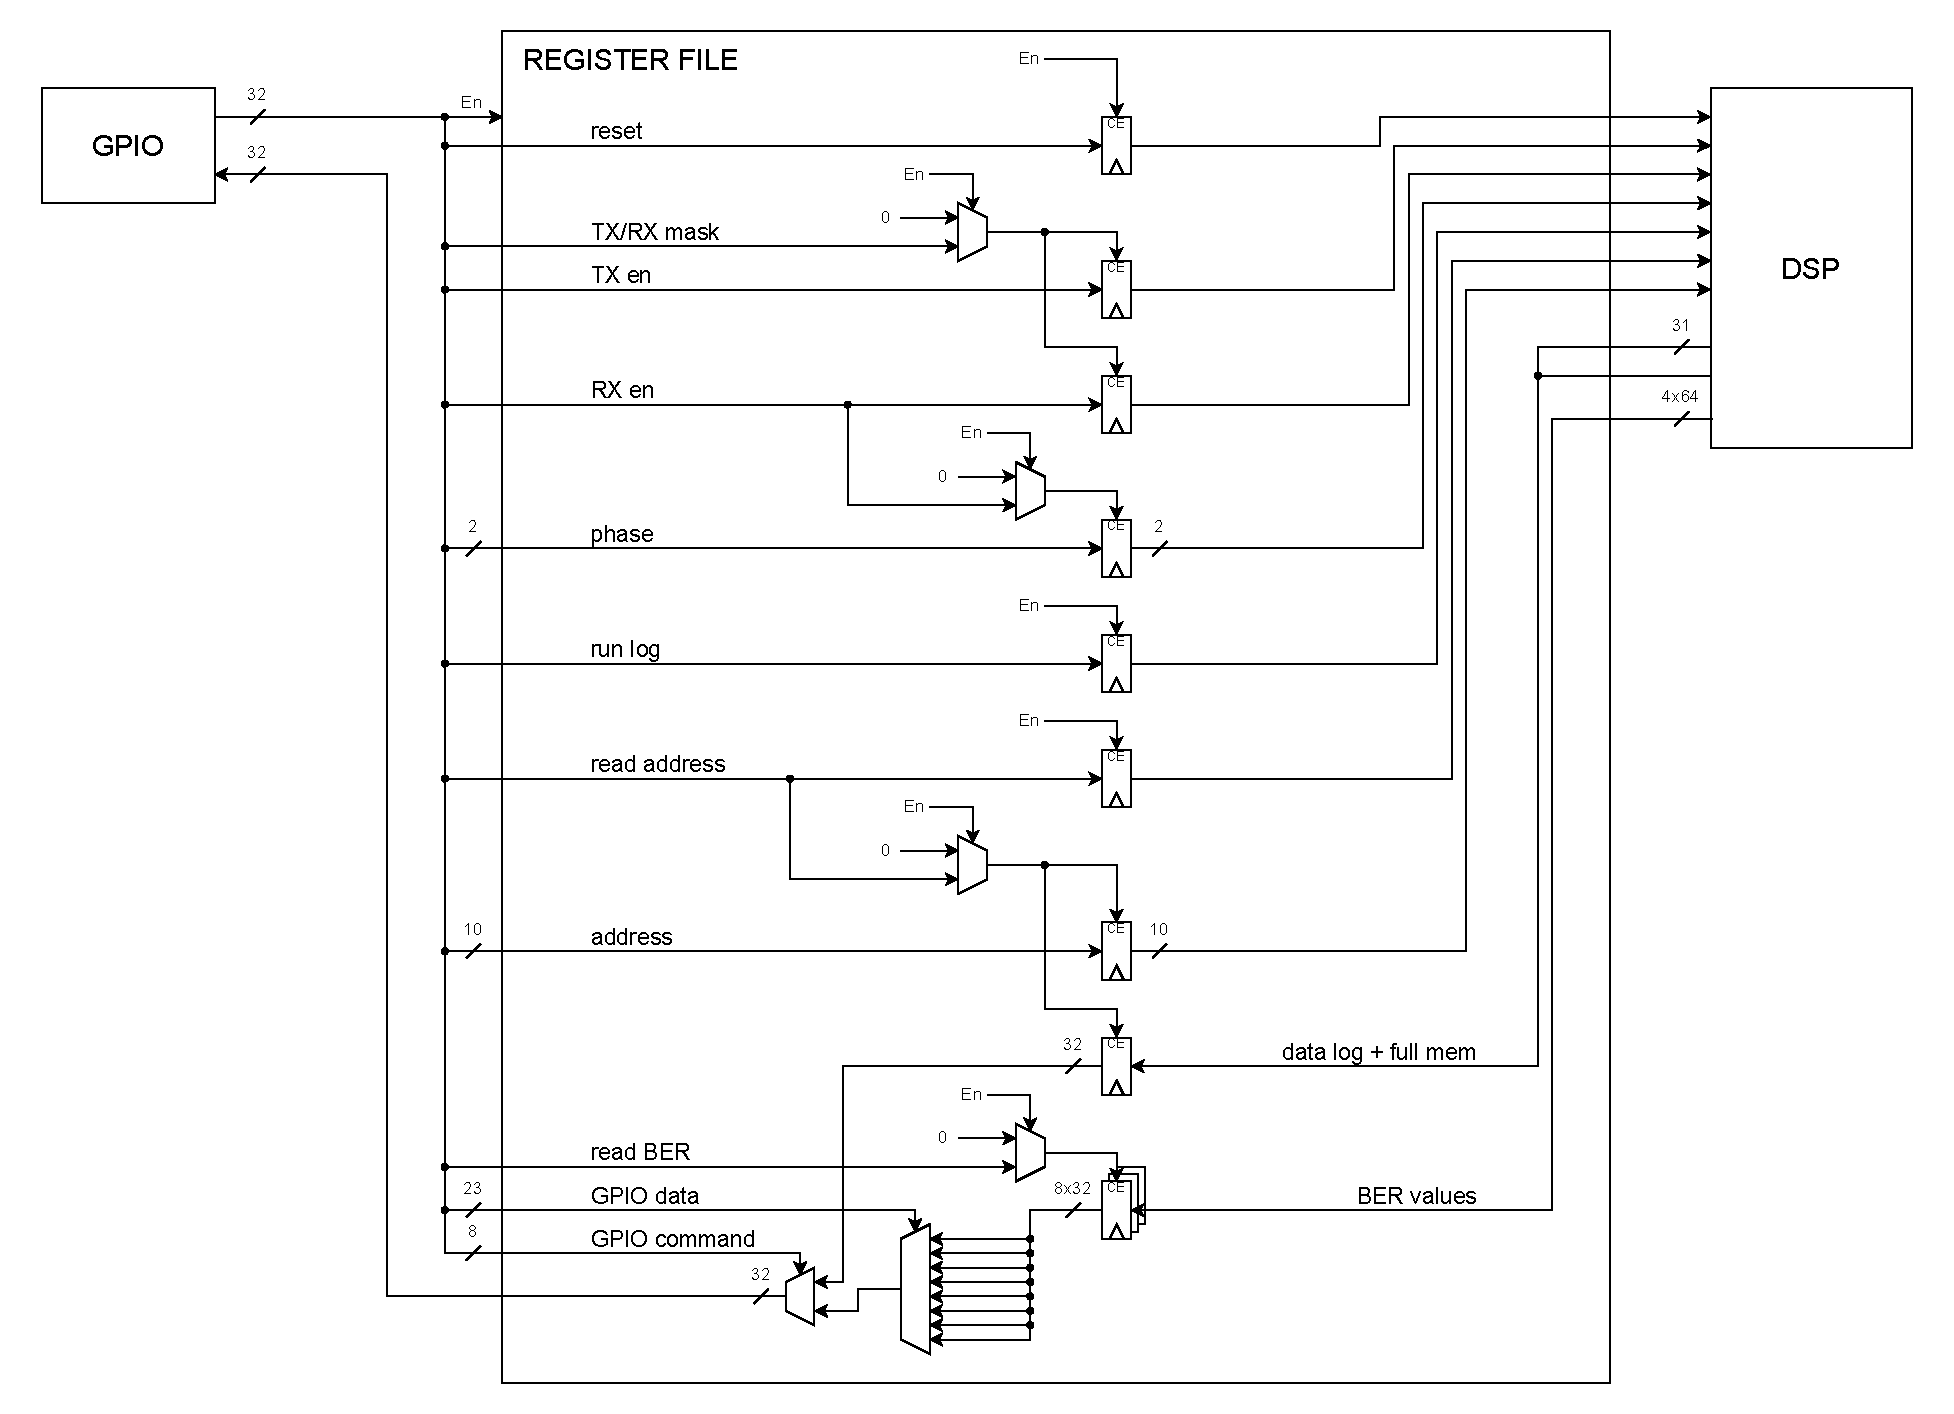
\includegraphics[width=\linewidth]{img/esq_rf.pdf}
    \caption{Arquitectura del register file, entre el periférico del GPIO y el DSP.}
    \label{fig:esq_rf}
\end{figure}

La salida del GPIO se divide según la \autoref{fig:dato_gpio}, donde cada campo se explica a continuación:

\begin{itemize}
    \item \textbf{GPIO Data}: en este campo se colocan valores auxiliares que acompañan a los valores del campo GPIO Command, en el caso de que corresponda.
    \item \textbf{Enable Command}: hay que levantar esta bandera para que se haga efectivo el envío del comando al register file, ya que este controla todos los registros.
    \item \textbf{GPIO Command}: contiene todos los bits de control que se desean enviar al DSP.
        \subitem \textbf{Reset DSP}: envía una señal de reset al DSP. Cuando se resetea con el botón de la placa, es el register file el que resetea al DSP con esta señal.
        \subitem \textbf{TX/RX Mask}: se levanta esta bandera para habilitar la actualización del estado del TX y el RX.
        \subitem \textbf{Enable TX}: actualiza el estado (encendido o apagado) del transmisor. Necesita que el bit TX/RX Mask esté levantado.
        \subitem \textbf{Enable RX}: actualiza el estado (encendido o apagado) del receptor. Si se lo enciende, se especifica la fase de muestreo en el campo GPIO Data. Necesita que el bit TX/RX Mask esté levantado.
        \subitem \textbf{Run Log}: el DSP comienza a almacenar datos en toda la memoria hasta que se llene.
        \subitem \textbf{Read address}: lee un dato de la memoria del DSP y lo envía al GPIO junto con la bandera de memoria llena en el bit más significativo. La dirección se especifica en el campo GPIO Data.
        \subitem \textbf{Read BER}: permite almacenar, en el GPIO de entrada, uno de los valores correspondientes al BER. Estos se deben especificar en el campo GPIO Data y pueden ser:
            \subsubitem \texttt{23'd0}: \emph{Error del canal I (parte alta)}
            \subsubitem \texttt{23'd1}: \emph{Error del canal I (parte baja)}
            \subsubitem \texttt{23'd2}: \emph{Símbolos totales del canal I (parte alta)}
            \subsubitem \texttt{23'd3}: \emph{Símbolos totales del canal I (parte baja)}
            \subsubitem \texttt{23'd4}: \emph{Error del canal Q (parte alta)}
            \subsubitem \texttt{23'd5}: \emph{Error del canal Q (parte baja)}
            \subsubitem \texttt{23'd6}: \emph{Símbolos totales del canal Q (parte alta)}
            \subsubitem \texttt{23'd7}: \emph{Símbolos totales del canal Q (parte baja)}
\end{itemize}

\begin{figure}[H]
    \centering
    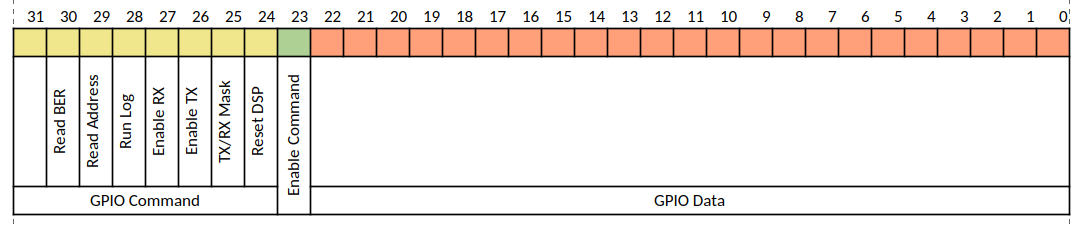
\includegraphics[width=0.9\linewidth]{img/dato_gpio.png}
    \caption{Campos de la salida del GPIO al register file.}
    \label{fig:dato_gpio}
\end{figure}

La idea de utilizar el campo Enable Command, es que el microprocesador escriba 3 veces un comando al GPIO de la siguiente manera:

\begin{enumerate}
    \item Escribe el campo GPIO Command y GPIO Data
    \item Escribe el bit Enable Command en 1
    \item Escribe el bit Enable Command en 0
\end{enumerate}

Con esto, el register file tiene 2 ciclos para mantener estable los bits del GPIO y así el comando se obtiene de forma segura. Esto es muy útil sobre todo en el caso de register files con cambios de dominio de reloj.

Para verificar este register file, se realizó un testbench que estimula la entrada con los comandos y el método antes mencionado, como si fuera el propio periférico GPIO. El flujo que realiza el testbench es:

\begin{enumerate}
    \item Resetear y luego encender el TX y el RX con la fase óptima.
    \item Leer todos los campos de BER pero solo la parte baja.
    \item Apagar y encender el RX con la peor fase.
    \item Leer todos los campos de BER.
    \item Habilitar el logueo en memoria.
    \item Leer todas las direcciones de la memoria.
\end{enumerate}

La lectura de algunos campos de BER se ve en la forma de onda de la \autoref{fig:sim_rf}, donde el módulo entrega el dato de los errores y símbolos totales del canal I y los errores del canal Q. Se puede ver, cuando se solicitan los símbolos del canal I, que el dato llega 1 ciclo después de levantar la bandera de habilitación, por lo que el dato luego tiene 1 ciclo para estabilizarse y leerse con el microprocesador. Como aclaración: en esta gráfica, \texttt{o\_led} indica que el sistema no está con reset y el transceptor está activo, \texttt{o\_led\_rgb\_0} indica que la memoria está vacía y no se la está leyendo, y \texttt{o\_led\_rgb\_1} indica que se encuentra en la fase 2 (óptima).

\begin{figure}[H]
    \centering
    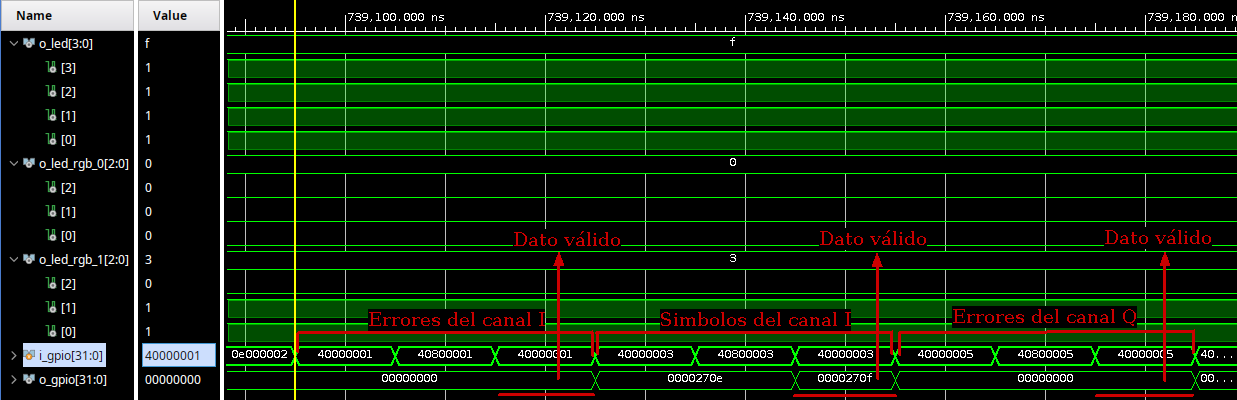
\includegraphics[width=\linewidth]{img/sim_rf.png}
    \caption{Forma de onda en la lectura de algunos campos de BER.}
    \label{fig:sim_rf}
\end{figure}

La \autoref{fig:sim_rf_ber_i} y \ref{fig:sim_rf_ber_q} muestran la lectura completa del BER en el canal I y Q cuando la fase es la errónea (fase 0). La parte alta de los valores es 0, ya que se simuló un tiempo corto; por otro lado, se puede ver que el valor del error y la cantidad total corresponden a instantes diferentes, ya que no se logró que el register file latchee al mismo tiempo los 8 registros, sin embargo, esta medición dio un resultado de $0.25$ como es de esperarse. Realizando los cálculos, se encontró que el máximo delay que hay entre el primer campo y el último es de 207 símbolos.

\begin{figure}[H]
    \centering
    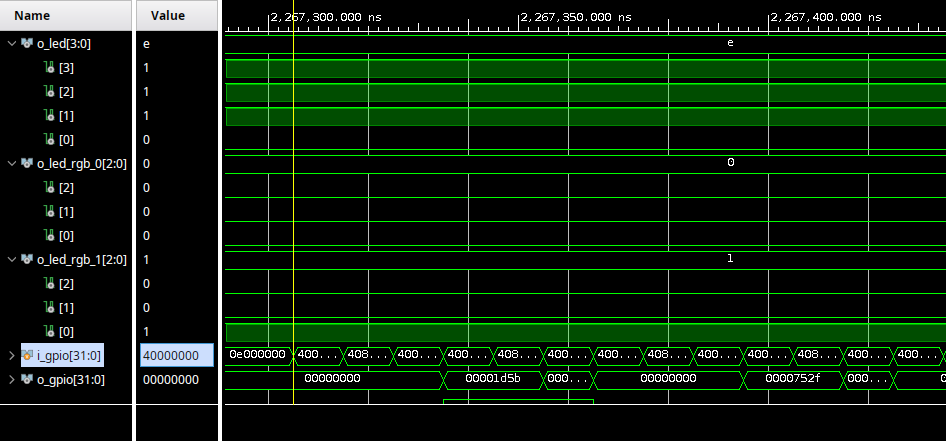
\includegraphics[width=0.9\linewidth]{img/sim_rf_ber_i.png}
    \caption{Forma de onda en la lectura de BER en el canal I.}
    \label{fig:sim_rf_ber_i}
\end{figure}

\begin{figure}[H]
    \centering
    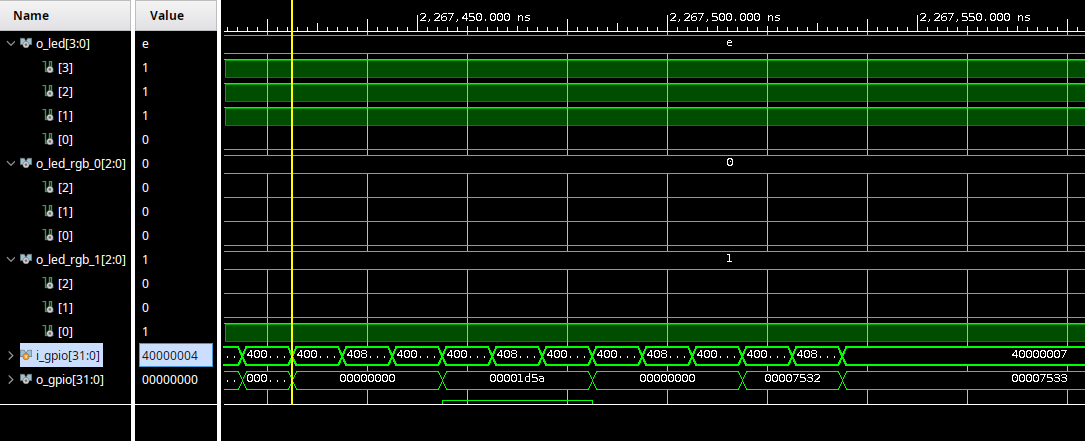
\includegraphics[width=0.9\linewidth]{img/sim_rf_ber_q.png}
    \caption{Forma de onda en la lectura de BER en el canal Q.}
    \label{fig:sim_rf_ber_q}
\end{figure}

Finalmente, se muestra en la \autoref{fig:sim_rf_mem} el proceso de lectura de la memoria llena. Se observa en \texttt{i\_gpio} que está solicitando la dirección 6, mientras que \texttt{o\_gpio} entrega los datos en I (bits 0 a 7) y en Q (bits 16 a 23), junto con la bandera de memoria llena (bit 31).

\begin{figure}[H]
    \centering
    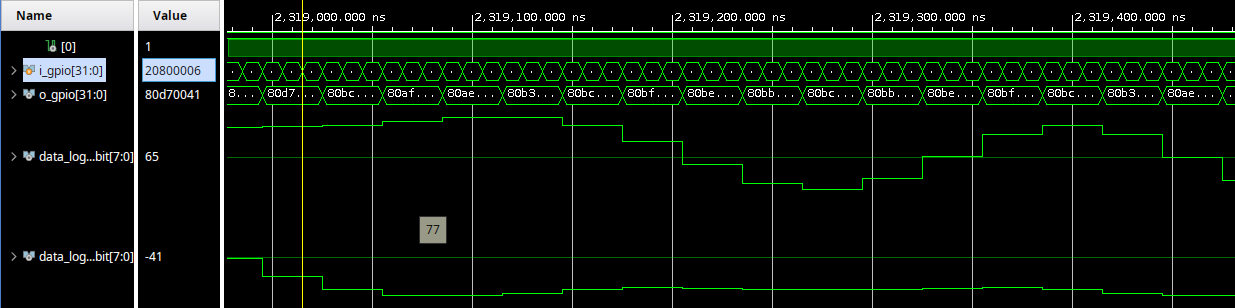
\includegraphics[width=\linewidth]{img/sim_rf_mem.png}
    \caption{Forma de onda en la lectura de la memoria. Al GPIO le llega el dato \texttt{41} en I, \texttt{d7} en Q y la memoria llena levantada, ya que se observa un \texttt{8}.}
    \label{fig:sim_rf_mem}
\end{figure}

\subsection{Microprocesador y Periféricos}

Se armó en Vivado el microprocesador MicroBlaze junto con el GPIO y el UART para luego instanciarlos en el top level. La arquitectura del microcontrolador completo se muestra en la \autoref{fig:esq_micro}. Debido a las limitaciones de memoria de la FPGA, se recomendó generar el micro con una memoria local de 32K, por lo que se puso en duda si es posible llegar a procesar los 32K datos de la memoria en el DSP.

\begin{figure}[H]
    \centering
    
\includegraphics[width=\linewidth]{img/esq_micro.png}
    \caption{Diagrama del microcontrolador instanciado en el diseño.}
    \label{fig:esq_micro}
\end{figure}

\subsubsection{Implementación del Módulo Completo}

El módulo top en forma resumida se puede observar en la \autoref{fig:esq_top}. Se instanció el VIO con varias salidas para observar el comportamiento a la hora de la implementación, también se quizo implementar el ILA, pero la herramienta arrojaba errores de timing.

\begin{figure}[H]
    \centering
    
\includegraphics[width=\linewidth]{img/esq_top.pdf}
    \caption{Esquema del diseño completo.}
    \label{fig:esq_top}
\end{figure}

La implementación arrojó los resultados de la \autoref{fig:imp_rep_1k}, como se tuvo éxito en la implementación con memoria de 1K, se pasó a cambiarla por 32K, lo que dio como resultado lo mostrado en la \autoref{fig:imp_rep_32k}. Se puede ver que el slack con 32K es menor que con 1K, pero finalmente no hay problemas de timing, por lo que se continuó el flujo con 32K. Puede notarse también el aumento significativo de bloques BRAM debido a este aumento de memoria.

\begin{figure}[H]
    \centering
    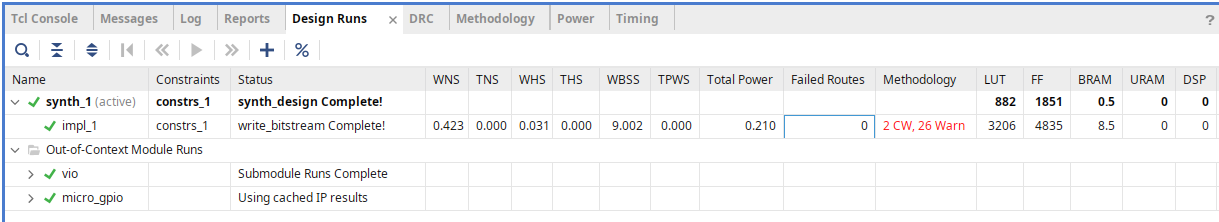
\includegraphics[width=\linewidth]{img/imp_rep_1k.png}
    \caption{Reporte de implementación con 1K de memoria.}
    \label{fig:imp_rep_1k}
\end{figure}

\begin{figure}[H]
    \centering
    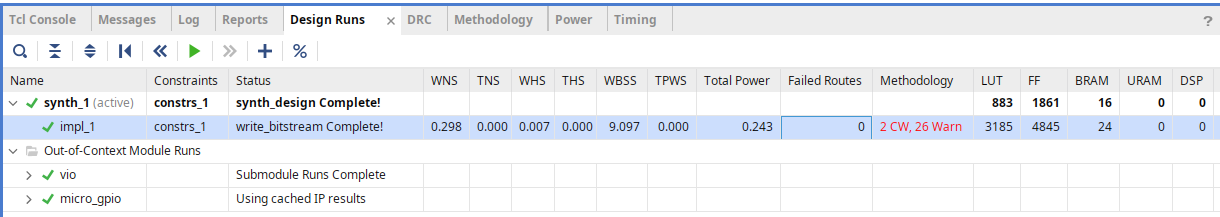
\includegraphics[width=\linewidth]{img/imp_rep_32k.png}
    \caption{Reporte de implementación con 32K de memoria.}
    \label{fig:imp_rep_32k}
\end{figure}

\begin{figure}[H]
    \centering

    \begin{minipage}{0.48\linewidth}
        \centering
        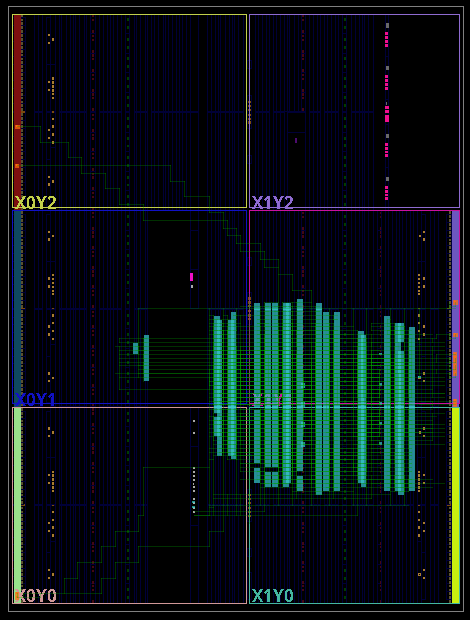
\includegraphics[width=0.8\linewidth]{img/imp_1k.png}
        \subcaption{Con 1K de memoria.}
        \label{fig:imp_1k}
    \end{minipage}
    \hfill
    \begin{minipage}{0.48\linewidth}
        \centering
        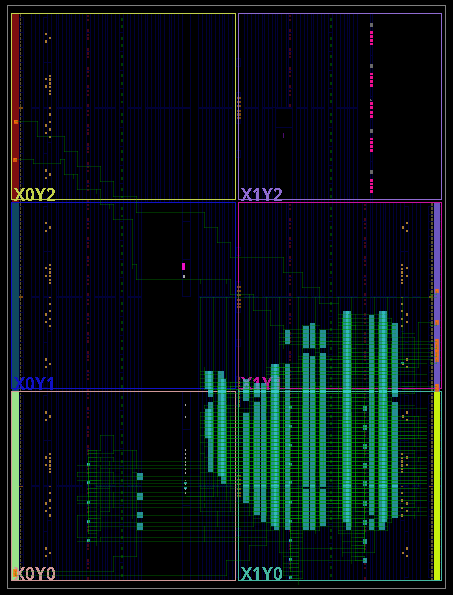
\includegraphics[width=0.8\linewidth]{img/imp_32k.png}
        \subcaption{Con 32K de memoria.}
        \label{fig:imp_32k}
    \end{minipage}

    \caption{Espacio utilizado en la FPGA.}
    \label{fig:imp}
\end{figure}

\subsection{Firmware}

El firmware programado para el micro se realizó de tal forma que se comunique con la PC de la misma forma que en el Laboratorio N°5. En este caso, escribe los GPIO 3 veces para mantener estables los comandos, como se explicó en la \autoref{sec:rf}.

En forma resumida, se programó el código en C según el diagrama de la \autoref{fig:esq_fw}.

\begin{figure}[H]
    \centering
    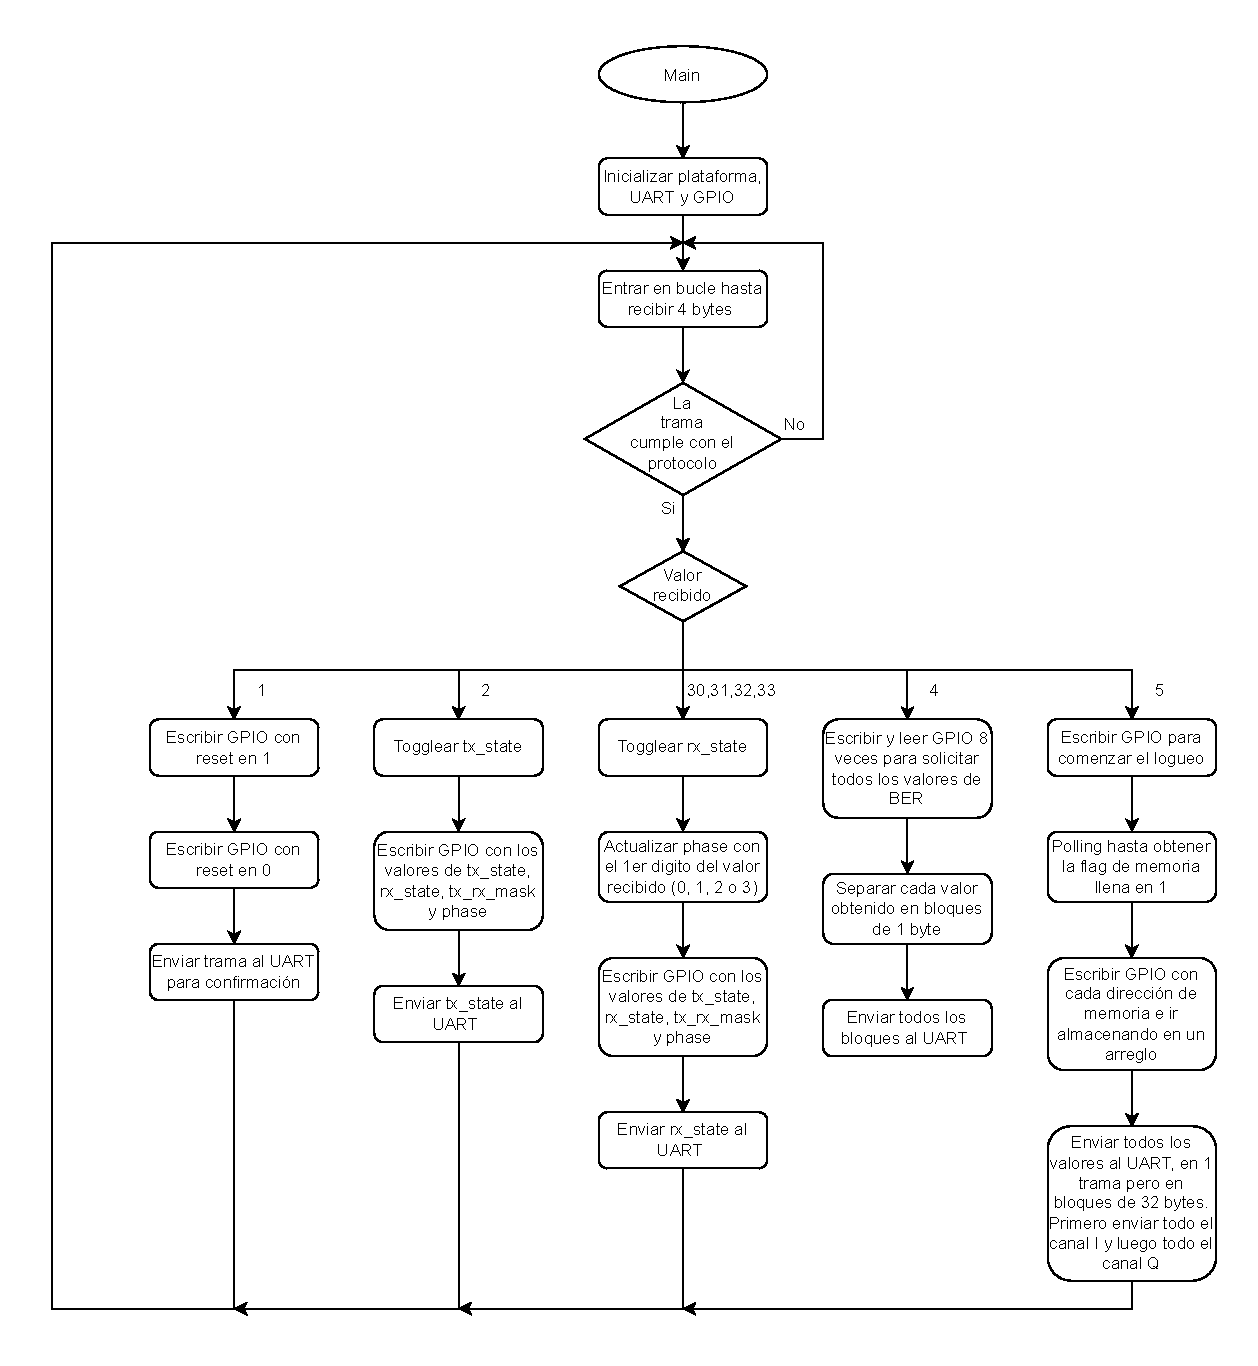
\includegraphics[width=\linewidth]{img/esq_fw.pdf}
    \caption{Diagrama de flujo del programa para el microprocesador.}
    \label{fig:esq_fw}
\end{figure}

\subsection{Python}

El script de Python para comunicarse con la FPGA fue mejorado con respecto al del Laboratorio N°5 para que pueda procesar de forma más completa las tramas recibidas de acuerdo al protocolo recomendado. Además de que se eliminó el tiempo de espera para que el resultado sea mostrado inmediatamente. El diagrama de flujo del script se muestra en la \autoref{fig:esq_python}.

\begin{figure}[H]
    \centering
    
\includegraphics[width=\linewidth]{img/esq_python.pdf}
    \caption{Diagrama de flujo del script de Python.}
    \label{fig:esq_python}
\end{figure}

\section{Resultados}

En un principio, todas las pruebas se realizaron con la BRAM física en 32K pero enviando 1K datos al micro, ya que el arreglo de 32K utilizado en el programa en C provocaba un error en el linker (archivo \texttt{lscript.ld}) debido a que la limitante era la memoria local del microprocesador. Una solución propuesta fue aumentar esta memoria local, editando el mapa de memoria en Vivado (\autoref{fig:addrmap}) y luego editar el linker para hacer coincidir el rango (\autoref{fig:linker}). La forma de haber logrado que el código compile fue aumentar el rango de la memoria local hasta 128K, lo cual la herramienta pudo implementar sin problemas en la FPGA. Sin embargo, a la hora de la prueba con el script de Python, la FPGA no enviaba ninguna trama por una razón que se desconoce, pero está claro que proviene de haber aumentado este rango. Otra solución fue llenar un arreglo pequeño con los datos y enviarlos por paquetes, pero debido a la falta de tiempo, esto no se implementó.

Por lo explicado anteriormente, se aclara que los resultados a continuación corresponden a una memoria de 8K, que es el máximo valor que pudo utilizarse.

\begin{figure}[b!]
    \centering
    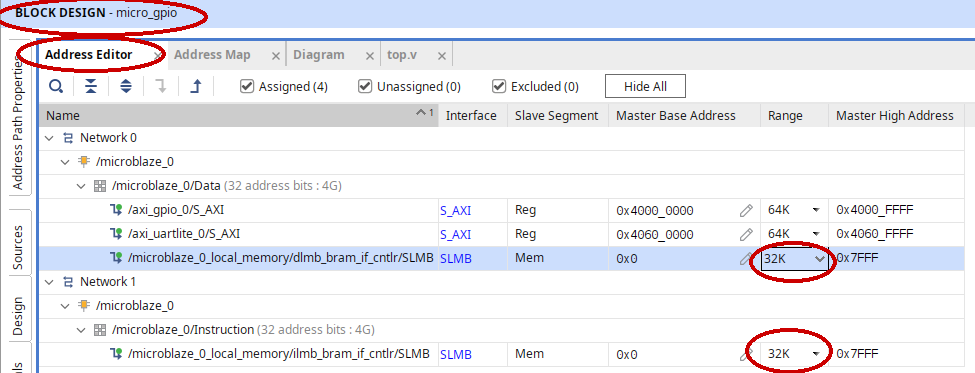
\includegraphics[width=\linewidth]{img/addrmap.png}
    \caption{Ventana para la edición de la memoria en el MicroBlaze.}
    \label{fig:addrmap}
\end{figure}

\begin{figure}[b!]
    \centering
    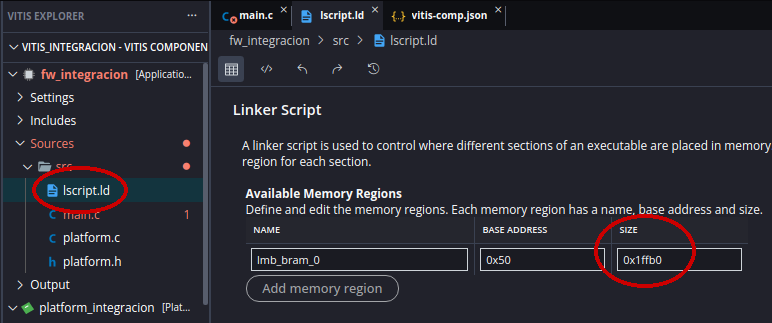
\includegraphics[width=\linewidth]{img/linker.png}
    \caption{Ventana para modificar la región de memoria en el linker.}
    \label{fig:linker}
\end{figure}

En la \autoref{fig:test1_init} se observa, a la izquierda, la interfaz principal del script conectado a la FPGA, y a la derecha, la interfaz del VIO. Las entradas del VIO son:

\begin{itemize}
    \item \texttt{probe\_in0[0]}: enganche del reloj del micro.
    \item \texttt{probe\_in0[1]}: reset del DSP.
    \item \texttt{probe\_in0[2]}: TX habilitado.
    \item \texttt{probe\_in0[3]}: RX habilitado.
    \item \texttt{probe\_in1[0]}: memoria llena.
    \item \texttt{probe\_in1[1]}: memoria leyéndose.
    \item \texttt{probe\_in1[2]}: iniciar logueo en la memoria.
    \item \texttt{probe\_in2}: fase de muestreo:
        \subitem \emph{Rojo}: fase 0.
        \subitem \emph{Verde}: fase 1.
        \subitem \emph{Rojo y verde}: fase 2.
        \subitem \emph{Azul}: fase 3.
    \item \texttt{probe\_in3}: bit recibido por el UART.
    \item \texttt{probe\_in4}: bit enviado por el UART.
\end{itemize}

El sistema inicia con el TX y el RX apagados, y se encienden insertando el número 2 y 3 en la consola. En la \autoref{fig:test2_tx} y \ref{fig:test3_rx} se muestra el encendido de estos, con la fase óptima. Si se desea cambiar de fase, debe apagarse el RX y volver a encenderse, como se muestra en la \autoref{fig:test4_ph0}.

Se realizó la lectura de BER para la fase óptima y la errónea (\autoref{fig:test5_ber_ph2} y \ref{fig:test6_ber_ph0}), mostrando resultados que coinciden con lo esperado: con la fase óptima se obtiene $BER = 0$ y con la errónea se obtiene $BER \approx 0.25$.

Un problema que se encontró fue cuando se vuelve a leer el BER luego de reiniciar el RX en la fase errónea (\autoref{fig:test7_ber_error}), donde es probable que aparezca $BER \approx 0.5$ en uno de los canales o los dos.

\begin{figure}[H]
    \centering
    \includegraphics[width=\linewidth]{img/test1_init.png}
    \caption{Interfaz de inicio del script.}
    \label{fig:test1_init}
\end{figure}

\begin{figure}[H]
    \centering
    \includegraphics[width=\linewidth]{img/test2_tx.png}
    \caption{Habilitación del transmisor.}
    \label{fig:test2_tx}
\end{figure}

\begin{figure}[H]
    \centering
    \includegraphics[width=\linewidth]{img/test3_rx.png}
    \caption{Habilitación del receptor con fase 2.}
    \label{fig:test3_rx}
\end{figure}

En la \autoref{fig:test8_mem} se puede ver cómo cambian los leds cuando se lee la memoria. El led de inicio de logueo se levanta y se baja; luego el led de lectura se levanta instantáneamente, ya que el micro espera que el bit de memoria llena se levante; y finalmente el bit de memoria llena se levanta.

Finalmente, se muestra en la \autoref{fig:test9_mem_luego_rst} cómo se bajan los leds correspondientes a la memoria cuando se reinicia el sistema.

El script guarda dos gráficos del log, uno completo con las 8K muestras y otro con zoom para observar mejor el comportamiento a la salida del filtro. Estos se muestran en la \autoref{fig:test10_plot_full} y \ref{fig:test11_plot}.

\begin{figure}[H]
    \centering
    \includegraphics[width=\linewidth]{img/test4_ph0.png}
    \caption{Reinicio del receptor con fase 0.}
    \label{fig:test4_ph0}
\end{figure}

\begin{figure}[H]
    \centering
    \includegraphics[width=\linewidth]{img/test5_ber_ph2.png}
    \caption{Lectura de BER con fase 2.}
    \label{fig:test5_ber_ph2}
\end{figure}

\begin{figure}[H]
    \centering
    \includegraphics[width=\linewidth]{img/test6_ber_ph0.png}
    \caption{Lectura de BER con fase 0.}
    \label{fig:test6_ber_ph0}
\end{figure}

\begin{figure}[H]
    \centering
    \includegraphics[width=\linewidth]{img/test7_ber_error.png}
    \caption{BER erróneo luego de reiniciar el RX.}
    \label{fig:test7_ber_error}
\end{figure}

\begin{figure}[H]
    \centering
    \includegraphics[width=\linewidth]{img/test8_mem.png}
    \caption{Almacenamiento de los últimos 8K datos.}
    \label{fig:test8_mem}
\end{figure}

\begin{figure}[H]
    \centering
    \includegraphics[width=\linewidth]{img/test9_mem_luego_rst.png}
    \caption{Reset del sistema luego de realizar el logueo.}
    \label{fig:test9_mem_luego_rst}
\end{figure}

\begin{figure}[H]
    \centering
    \includegraphics[width=\linewidth]{img/test10_plot_full.png}
    \caption{Grafico completo del logueo.}
    \label{fig:test10_plot_full}
\end{figure}

\begin{figure}[H]
    \centering
    \includegraphics[width=\linewidth]{img/test11_plot.png}
    \caption{Gráfico del logueo con zoom.}
    \label{fig:test11_plot}
\end{figure}

\section{Conclusiones}

Se implementó una memoria al DSP del Laboratorio N°4 y se lo integró con el microcontrolador del Laboratorio N°5 para ser controlado con un script de Python. El control pudo realizarse con éxito, permitiendo obtener una BER de aproximadamente $0.25$ en la fase errónea y BER de 0 en las demás fases. Sin embargo, al reiniciar el receptor con fase errónea, el BER sube repentinamente y no se encontró la causa. En cuanto a la lectura de memoria, solo se pudo obtener un logueo de hasta 8K muestras, mientras que el hardware del DSP sí puede escribir en una memoria de 32K. Como trabajo a futuro se propone modificar el programa en C para realizar la recepción de estas muestras por paquetes para así aprovechar toda la memoria.

\newpage
\appendix

\section{Archivos y Códigos} \label{appx:archivos}

Todos los códigos del trabajo se encuentran en el siguiente link:

\noindent
\url{https://github.com/Ruben-Zuniga/Introduccion-al-Disenio-Digital/tree/main/TP6}

La organización del repositorio adjunto es el siguiente:

\begin{itemize}
    \item \emph{com\_serie\_tp6.py}: el script de Python utilizado.
    \item \emph{main.c}: el programa en C del microprocesador.
    \item \emph{rtl}: contiene todos los módulos en Verilog del hardware.
    \item \emph{tb}: contiene dos testbenches: uno que funciona con el register file (el utilizado en este trabajo) y uno que no.
    \item \emph{latex}: contiene todos los códigos en Latex e imágenes del informe.
    \item \emph{drawio}: proyectos realizados para generar los esquemas en este informe.
    \item \emph{Arty\_Master\_v2.xdc}: el constraint para la implementación.
\end{itemize}

% \begin{equation}
%     \boxed{
%         1 = 2
%     }
% \end{equation}

% \begin{table}[H]
%     \centering
%
%     \begin{tabular}{lcc}
%         \textbf{A} & \textbf{B} & \textbf{C} \\
%         \hline\hline
%         A & B & C \\
%         A & B & C \\
%         \hline
%     \end{tabular}
%
%     \caption{cap.}
%     \label{tab:tab}
% \end{table}

% \begin{table}[H]
%     \centering
%     \begin{tblr}{
%         row{1} = {Titulo},
%         column{1} = {Titulo},
%         colspec = {Q[l] Q[c] Q[c]},
%         vlines,
%         hlines,
%         width=\linewidth
%     }
%         A & B & C \\
%         A & B & C \\
%         A & B & C \\

%     \end{tblr}
%     \caption{cap.}
%     \label{tab:tab}
% \end{table}

% \begin{figure}[H]
%     \centering
%     \includegraphics[width=0.85\linewidth]{img/sim.png}
%     \caption{cap.}
%     \label{fig:fig}
% \end{figure}

% \begin{figure}[H]
%     \centering

%     \begin{minipage}{0.48\linewidth}
%         \centering
%         \includegraphics[width=1\linewidth]{img/ondas_completo1.png}
%     \end{minipage}
%     \hfill
%     \begin{minipage}{0.48\linewidth}
%         \centering
%         \includegraphics[width=1\linewidth]{img/ondas_completo2.png}
%     \end{minipage}

%     \caption{cap.}
%     \label{fig:fig}
% \end{figure}

% \begin{figure}[H]
%     \centering

%     \begin{minipage}{\linewidth}
%         \centering
%         
\includegraphics[width=1\linewidth]{img/fulgor_logo.jpg}
%         \subcaption{cap.}
%         \label{fig:fig}
%     \end{minipage}
    
%     \begin{minipage}{\linewidth}
%         \centering
%         
\includegraphics[width=1\linewidth]{img/fulgor_logo.jpg}
%         \subcaption{cap.}
%         \label{fig:fig}
%     \end{minipage}
    
%     \begin{minipage}{\linewidth}
%         \centering
%         
\includegraphics[width=1\linewidth]{img/fulgor_logo.jpg}
%         \subcaption{cap.}
%         \label{fig:fig}
%     \end{minipage}

%     \caption{cap.}
%     \label{fig:fig}
% \end{figure}